% -*- TeX:UK -*-
\chapter{Vector arithmetic}
\begin{refsection}

\abstract{Vectors and arrays are probably the most common data structures. However, in \texttt{Pascal} their use is not comfortable, as their size needs to be determined at compile-time. This makes it difficult to write reusable code. In \Name{Wirth}'s \texttt{Pascal} definition \parencite{Jen-74} there were \textbf{conformant arrays} for this purpose, however, these were not implemented in most \texttt{Pascal} dialects, including \texttt{Object Pascal}.}

One can define arrays large enough for all purposes, and then use only whatever part is actually required. However, this is memory-expensive. Under 16-bit operating systems like DOS the data segment was limited to \SI{64}{kB}, equivalent to about \num{8000} elements. Even under modern \SI{64}{Bit} operating systems and compilers, this problem isn't solved, because the stack (required for passing of variables to functions and procedures) still has this limit.

In addition, with this method the size of the array has to be passed with the data structure, a possible source of errors. Thus, it would be useful to have size information in the structure itself:

\begin{lstlisting}[caption=]
TYPE VectorStruc = RECORD
                     Columns : WORD;
                     Data : ARRAY [1..MaxVector] of float;
                   END;
\end{lstlisting}
and then use pointers to pass data to functions, in order to save stack space and -- in \SI{16}{Bit} systems -- to have the data on the heap to avoid space problems as much as possible:
\begin{lstlisting}[caption=]
    VectorTyp = ^VectorStruc;
\end{lstlisting}

This leads to the following interface
\begin{lstlisting}[caption=Interface of unit Vector]
  UNIT Vector;

  INTERFACE

  USES Math, mathfunc;

  CONST
    MaxVector = 8000;             // PowerOfTwo[16] DIV SizeOf(float);
    VectorError: BOOLEAN = FALSE; // toggle IF error occurs.


  TYPE
    VectorStruc = RECORD
      Length: WORD;
      Data: ARRAY [1..MaxVector] OF float;
    END;
    VectorTyp = ^VectorStruc;

  PROCEDURE CreateVector(VAR Vec: VectorTyp; Length: WORD; Value: float);

  PROCEDURE DestroyVector(VAR Vec: VectorTyp);

  PROCEDURE ReadVector(VAR Vec: VectorTyp; MedStr: STRING);

  PROCEDURE WriteVector(MedStr: STRING; CONST Vec: VectorTyp; ValidFigures: BYTE);

  FUNCTION VectorLength(CONST Vec: VectorTyp): WORD;

  FUNCTION GetVectorElement(CONST Vec: VectorTyp; n: WORD): float;

  PROCEDURE SetVectorElement(VAR Vec: VectorTyp; n: WORD; c: float);

  PROCEDURE CopyVector(CONST Source: VectorTyp; VAR Dest: VectorTyp);

  PROCEDURE LoadConstant(VAR Vec: VectorTyp; C: float);

  PROCEDURE AddConstant(VAR A: VectorTyp; C: float);

  PROCEDURE SubConstant(VAR A: VectorTyp; C: float);

  PROCEDURE MulConstant(VAR A: VectorTyp; C: float);

  PROCEDURE DivConstant(VAR A: VectorTyp; C: float);

  PROCEDURE VectorAdd(CONST A, B: VectorTyp; VAR C: VectorTyp);

  PROCEDURE VectorSub(CONST A, B: VectorTyp; VAR C: VectorTyp);

  FUNCTION VectorInnerProduct(CONST A, B: VectorTyp): float;

  FUNCTION TotalSum(CONST Vec: VectorTyp): float;

  FUNCTION NeumaierSum(CONST A: VectorTyp): float;

  FUNCTION TotalProduct(CONST Vec: VectorTyp): float;

  FUNCTION ActualElements(CONST A: VectorTyp): WORD;

  FUNCTION VectorSignum(Vec: VectorTyp): INTEGER;

  FUNCTION FindLargest(Vec: VectorTyp): float;
  { returns largest element of vector }

  FUNCTION FindSmallest(Vec: VectorTyp): float;

  FUNCTION FindLargestAbsolute(Vec: VectorTyp): float;

  FUNCTION FindSmallestAbsolute(Vec: VectorTyp): float;

  PROCEDURE Scale(VAR Vec: VectorTyp; min, max: float);

  PROCEDURE Centre(VAR Vec: VectorTyp);

  FUNCTION VectorAngle(CONST A, B: VectorTyp): float;

  { ------------ Vector norms, normalisation  ------------------- }

  FUNCTION VectorEuklidianNorm(CONST Vec: VectorTyp): float;

  FUNCTION VectorMaximumNorm(CONST Vec: VectorTyp): float;

  FUNCTION VectorAbsoluteSumNorm(CONST Vec: VectorTyp): float;

  PROCEDURE NormaliseVector(VAR Vec: VectorTyp; Norm: float);

  { ---------------- Elemente sortieren ---------------- }

  PROCEDURE ShellSort(VAR t: VectorTyp);

  { ------------------ Distance ------------------------ }

  FUNCTION SquaredEuklidianDistance(CONST A, B: VectorTyp;

  { ---------------------------------------------------- }

  IMPLEMENTATION

  VAR
    CH: CHAR;
\end{lstlisting}
The mechanism of error handling is the same as discussed for unit \texttt{MathFunc}.

\section{Generation and destruction of vectors}

This unit is written for data handling in sciences. By convention, we will use elements \(1\ldots n \) in this unit, rather then \(0\ldots n-1 \), as some other programmers (who come from pure math) do.

Vectors contain \texttt{Length} times the data space required to store a float number plus the size of the word variable \texttt{Length}. As a matter of fact, 6 additional bytes are also required. This amount of memory needs to be reserved when a vector is created, and released again when it is destroyed. If not enough memory is available, the attempt is aborted and an error message is produced. The calling routine is informed about the error situation by the flag \texttt{VectorError}:
\begin{lstlisting}[caption=eneration and destruction of vectors]
  PROCEDURE CreateVector(VAR Vec: VectorTyp; Length: WORD; Value: float);

  VAR
    i: WORD;

  BEGIN
    TRY
      GetMem(Vec, Length * SizeOf(float) + SizeOf(WORD) + 6);
    EXCEPT
      CH := WriteErrorMessage(' Not enough memory to create vector');
      VectorError := true;
      EXIT;
    END;
    Vec^.Length := Length;
    FOR i := 1 TO Length DO
      Vec^.Data[i] := Value;
  END;

  PROCEDURE DestroyVector(VAR Vec: VectorTyp);

  VAR
    x: WORD;

  BEGIN
    x := Vec^.Length * SizeOf(float) + SizeOf(WORD) + 6;
    FreeMem(Vec, x);
  END;


  PROCEDURE ReadVector(VAR Vec: VectorTyp; MedStr: STRING);

  VAR
    j, l: WORD;
    Medium: TEXT;

  BEGIN
    Assign(Medium, MedStr);
    Reset(Medium);
    IF IOResult <> 0 THEN
    BEGIN
      CH := WriteErrorMessage(' File with vector not found');
      VectorError := true;
      EXIT;
    END;
    ReadLn(Medium, l);
    FOR j := 1 TO l DO
    BEGIN
      IF EoF(Medium) THEN
      BEGIN
        CH := WriteErrorMessage(' Unknown file format');
        VectorError := true;
        EXIT;
      END;
      ReadLn(Medium, Vec^.Data[j]);
      IF IOResult <> 0 THEN
      BEGIN
        CH := WriteErrorMessage(' Unknown file format');
        VectorError := true;
        EXIT;
      END;
    END;
    Close(Medium);
  END;


  PROCEDURE WriteVector(MedStr: STRING; CONST Vec: VectorTyp; ValidFigures: BYTE);

  VAR
    j: WORD;
    Medium: TEXT;

  BEGIN
    Assign(Medium, MedStr);
    Rewrite(Medium);
    Writeln(Medium, Vec^.Length);
    FOR j := 1 TO Vec^.Length DO
      Write(Medium, FloatStr(Vec^.Data[j], ValidFigures), ' ');
    Close(Medium);
  END;
\end{lstlisting}

It is not possible to copy these vectors by \(\AbsVec{a} = \AbsVec{b} \), rather, the following procedure needs to be used:

\begin{lstlisting}[caption=]
  PROCEDURE CopyVector(CONST Source: VectorTyp; VAR Dest: VectorTyp);

  VAR
    i, n: WORD;

  BEGIN
    n := VectorLength(Source);
    TRY
      GetMem(Dest, n * SizeOf(float) + SizeOf(WORD) + 6);
    EXCEPT
      CH := WriteErrorMessage(' Copy vector: Not enough memory to create copy');
      VectorError := true;
      EXIT;
    END;
    CreateVector(Dest, n, 0.0);
    FOR i := 1 TO n DO
      SetVectorElement(Dest, i, GetVectorElement(Source, i));
  END;
\end{lstlisting}

\section{Accesing and changing data in vectors}

The following routines provide opaque access to the information in vectors, that is, they work irrespective on how the vector is implemented. Access from outside of this unit should always use these routines. To save memory and execution time, unchanged vectors are given the key word \texttt{const} in the definition of routines, this prevents copying of these structures (call by reference instead of call by value). In older \texttt{Pascal} dialects use \texttt{var} for the same purpose:
\begin{lstlisting}[caption=Accesing and changing data in vectors]
  FUNCTION VectorLength(CONST Vec: VectorTyp): WORD;

  BEGIN
    Result := Vec^.Length;
  END;


  FUNCTION GetVectorElement(CONST Vec: VectorTyp; n: WORD): float;

  VAR
    s1, s2: STRING;

  BEGIN
    IF ((n <= VectorLength(Vec)) AND (n > 0))
      THEN
        Result := Vec^.Data[n]
      ELSE
        BEGIN
          Str(n: 4, s1);
          Str(VectorLength(Vec): 4, s2);
          CH := WriteErrorMessage(' Attempt to read non-existend vector element No ' +
                 s1 + ' of ' + s2);
        END;
  END;


  PROCEDURE SetVectorElement(VAR Vec: VectorTyp; n: WORD; C: float);

  BEGIN
    IF ((n <= VectorLength(Vec)) AND (n > 0)) THEN
      Vec^.Data[n] := C
    ELSE
      BEGIN
        CH := WriteErrorMessage(' Attempt to write to non-existend vector element');
        VectorError := true;
      END;
  END;
\end{lstlisting}

\section{Calculation with vectors}

\subsection{Calculations using one vector and a constant number as argument}

\begin{lstlisting}[caption=Calculations using one vector and a constant number as argument]
  PROCEDURE LoadConstant(VAR Vec: VectorTyp; C: float);

  VAR
    i, n: WORD;

  BEGIN
    n := VectorLength(Vec);
    IF (n = 0) THEN EXIT;
    FOR i := 1 TO n DO
      SetVectorElement(Vec, i, C);
  END;


  PROCEDURE AddConstant(VAR A: VectorTyp; C: float);

  VAR
    i, n: WORD;

  BEGIN
    n := VectorLength(A);
    IF (n = 0) THEN EXIT;
    FOR i := 1 TO n DO
      SetVectorElement(A, i, GetVectorElement(A, i) + C);
  END;


  PROCEDURE SubConstant(VAR A: VectorTyp; C: float);

  VAR
    i, n: WORD;

  BEGIN
    n := VectorLength(A);
    IF (n = 0) THEN EXIT;
    FOR i := 1 TO n DO
      SetVectorElement(A, i, GetVectorElement(A, i) - C);
  END;



  PROCEDURE MulConstant(VAR A: VectorTyp; C: float);

  VAR
    i, n: WORD;

  BEGIN
    n := VectorLength(A);
    IF (n = 0) THEN EXIT;
    FOR i := 1 TO n DO
      SetVectorElement(A, i, GetVectorElement(A, i) * C);

  END;


  PROCEDURE DivConstant(VAR A: VectorTyp; C: float);

  VAR
    i, n: WORD;

  BEGIN
    n := VectorLength(A);
    IF (n = 0) THEN EXIT;
    FOR i := 1 TO n DO
      SetVectorElement(A, i, GetVectorElement(A, i) / C);
  END;
\end{lstlisting}

\subsection{Routines that take two vectors and calculate a third}

\subsubsection{Addition and subtraction of vectors}

\begin{lstlisting}[caption=]
  PROCEDURE VectorAdd(CONST A, B: VectorTyp; VAR C: VectorTyp);

  VAR
    i, n: WORD;

  BEGIN
    n := VectorLength(A);
    IF (n = 0) OR (n <> VectorLength(B))
      THEN
        BEGIN
          CH := WriteErrorMessage(' Addition of vectors: vectors of different lengths');
          VectorError := true;
          EXIT;
        END;
    CreateVector(C, n, 0.0);
    FOR i := 1 TO n DO
      SetVectorElement(C, i, GetVectorElement(A, i) + GetVectorElement(B, i));
  END;


  PROCEDURE VectorSub(CONST A, B: VectorTyp; VAR C: VectorTyp);

  VAR
    i, n: WORD;

  BEGIN
    n := VectorLength(A);
    IF (n = 0) OR (n <> VectorLength(B))
      THEN
        BEGIN
          CH := WriteErrorMessage(' Subtraction of vectors: vectors of different lengths');
          VectorError := true;
          EXIT;
        END;
    CreateVector(C, n, 0.0);
    FOR i := 1 TO n DO
      SetVectorElement(C, i, GetVectorElement(A, i) - GetVectorElement(B, i));
  END;
\end{lstlisting}


\subsection{Functions that take a Vector and produce a number }

\subsubsection{Sum over all vector elements}

The sum of all elements of \AbsVec{x} (S = \(\sum_{i=1}^n{\AbsVec{x}_i} \)) is used to calculate the arithmetic mean of the elements \(\bar{\AbsVec{x}} = S/n \), that is:

\begin{lstlisting}[caption=Grand total of vector elements]
  FUNCTION TotalSum(CONST Vec: VectorTyp): float;

  VAR
    i, n: WORD;
    x: float;

  BEGIN
    n := VectorLength(Vec);
    IF (n = 0)
      THEN
        BEGIN
          TotalSum := 0;
          EXIT;
        END;
    x := 0;
    FOR i := 1 TO n DO
      IF IsNaN(GetVectorElement(Vec, i))
        THEN
        ELSE x := x + GetVectorElement(Vec, i);
    Result := x;
  END;
\end{lstlisting}

The problem with this na{\"i}ve implementation is that with floating point arithmetic there may be a catastrophic accumulation of error when the summands have very different orders of magnitude. For example, the sum of \((1.0, +\num{e100}, 1.0, \num{-e100}) \) obviously should be \num{2.0}, but above routine will yield \num{0.0} when performed in IEEE double precision. \Name{Neumaier}'s compensated summation algorithm calculates and sums the rounding error of each step, the sum is added to the final result. This reduces the relative error from \(\mathbf{O}(n \epsilon) \) to \(\mathbf{O}(\epsilon) \), unless \skalar{n} becomes significant compared to \(1/\epsilon \)  (\num{e16} in IEEE double precision arithmetic).

\begin{lstlisting}[caption=Compensated summation]
  FUNCTION NeumaierSum(CONST A: VectorTyp): float;

  VAR
    Sum, c, t, x: float;
    i, j: WORD;

  BEGIN
    IF (VectorLength(A) = 0)
      THEN
        BEGIN
          NeumaierSum := 0;
          EXIT;
        END;
    i := 1;
    REPEAT     // search FOR the first non-NaN element
      Sum := GetVectorElement(A, i);
      INC(i)
    UNTIL NOT (IsNaN(Sum));
    c := 0.0;
    FOR j := i TO VectorLength(A) DO
      IF IsNaN(GetVectorElement(A, j))
        THEN
        ELSE
          BEGIN
            x := GetVectorElement(A, j);
            t := Sum + x;
            IF Abs(Sum) >= Abs(x)
              THEN c := c + ((Sum - t) + x)   // LOW-order digits OF A(j) are lost
              ELSE c := c + ((x - t) + Sum);  // LOW-order digits OF Sum are lost
            Sum := t;
          END;
    Result := Sum + c;
  END;
\end{lstlisting}

\subsubsection{Product over all vector elements}

Similarly, the overall product \(P = \prod_{i=1}^n{\AbsVec{x}_i} \) is used for the harmonic mean \(\tilde{\AbsVec{x}} = \sqrt[n]{P} \):

\begin{lstlisting}[caption=Product of all vector elements]
  FUNCTION TotalProduct(CONST Vec: VectorTyp): float;

  VAR
    i, n: WORD;
    x: float;

  BEGIN
    n := VectorLength(Vec);
    IF (n = 0)
      THEN
        BEGIN
          TotalProduct := 0;
          EXIT;
        END;
    x := 0;
    FOR i := 1 TO n DO
      IF IsNaN(Vec^.Data[i])
        THEN
        ELSE x := x + Ln(GetVectorElement(Vec, i));
    TotalProduct := Exp(x);
  END;
\end{lstlisting}
For vectors with many large elements or very large length, it can be useful to calculate the total product from the sum of the logarithms of vector elements to avoid floating point overflow. \Name{Neumaier} correction is not required in such cases as the logarithms will be of similar magnitude.

\subsection{Properties of a vector}

A vector is positive, if \( \AbsVec{x}_i \geq 0 \), it is strictly positive if \( \AbsVec{x}_i > 0\ \forall\ i \in 1\ldots n \). \texttt{VectorSignum} returns \num{1} for strictly positive, \num{0} for positive and \num{-1} for vectors containing negative elements.

\begin{lstlisting}[caption=Signum of vector]
 FUNCTION VectorSignum(Vec: VectorTyp): INTEGER;

  VAR
    x: float;
    i: WORD;

  BEGIN
    VectorSignum := 1;
    FOR i := 1 TO VectorLength(Vec) DO
      BEGIN
        x := GetVectorElement(Vec, i);
        IF IsNaN(x)
          THEN
          ELSE
            CASE signum(x) OF
              -1: BEGIN
                    VectorSignum := -1; // one negative element IS enough
                    EXIT;
                  END;
              0: BEGIN
                   Result := 0; // continue IN CASE a negative element comes later
                 END;
              1: BEGIN
                  // do nothing
                 END;
            END; { case }
      END; { for }
  END;
\end{lstlisting}

\begin{lstlisting}[caption=Smallest and largest absolute value]
  FUNCTION FindLargestAbsolute(Vec: VectorTyp): float;

  VAR
    i: WORD;
    a: float;

  BEGIN
    a := GetVectorElement(Vec, 1);
    FOR i := 2 TO VectorLength(Vec) DO
      IF Abs(a) < Abs(GetVectorElement(Vec, i))
        THEN a := GetVectorElement(Vec, i);
    Result := a;
  END;


  FUNCTION FindSmallestAbsolute(Vec: VectorTyp): float;

  VAR
    i: WORD;
    a: float;

  BEGIN
    a := GetVectorElement(Vec, 1);
    FOR i := 2 TO VectorLength(Vec) DO
      IF Abs(a) > Abs(GetVectorElement(Vec, i))
        THEN a := GetVectorElement(Vec, i);
    Result := a;
  END;


  FUNCTION FindLargest(Vec: VectorTyp): float;

  VAR
    i: WORD;
    a: float;

  BEGIN
    a := GetVectorElement(Vec, 1);
    FOR i := 2 TO VectorLength(Vec) DO
      IF a < GetVectorElement(Vec, i)
        THEN a := GetVectorElement(Vec, i);
    Result := a;
  END;


  FUNCTION FindSmallest(Vec: VectorTyp): float;

  VAR
    i: WORD;
    a: float;

  BEGIN
    a := GetVectorElement(Vec, 1);
    FOR i := 2 TO VectorLength(Vec) DO
      IF a > GetVectorElement(Vec, i)
        THEN a := GetVectorElement(Vec, i);
    Result := a;
  END;
\end{lstlisting}

\subsection{Vector norms}\label{text:Norm}


\subsubsection{\Name{Euklid}ian norm of a vector}

The length or \Name{Euklid}ian norm of a vector is \(\ell_2 = ||\AbsVec{x}||_2 = \sqrt{\sum_{i=1}^n{\AbsVec{x}_i^2}} \):

\begin{lstlisting}[caption=\Name{Euklid}ian norm]
  FUNCTION VectorEuklidianNorm(CONST Vec: VectorTyp): float;

  VAR
    i, n: WORD;
    x: VectorTyp;

  BEGIN
    n := VectorLength(Vec);
    IF (n = 0)
      THEN
        BEGIN
          Result := 0;
          EXIT;
        END;
    CreateVector(x, n, 0.0);
    IF VectorError THEN EXIT;
    FOR i := 1 TO Vec^.Length DO
      SetVectorElement(x, i, Sqr(GetVectorElement(Vec, i)));
    VectorEuklidianNorm := Sqrt(NeumaierSum(x)); // avoid rounding error during summation
    DestroyVector(x);
  END;
\end{lstlisting}

\subsubsection{\Name{Tschebyschew}-norm}

The maximum (\Name{Tschebyschew}-, chess board-) norm \(||\AbsVec{x}||_\infty = \max_{i=1\ldots n}(|\AbsVec{x}_i|) \) is the absolute largest element of \AbsVec{x}:

\begin{lstlisting}[caption=Maximum norm]
  FUNCTION VectorMaximumNorm(CONST Vec: VectorTyp): float;

  VAR
    Max, Element: float;
    i: WORD;

  BEGIN
    IF (VectorLength(Vec) = 0)
      THEN
        BEGIN
          Result := 0;
          EXIT;
        END;
    Max := -1e300;
    FOR i := 1 TO VectorLength(Vec) DO
      BEGIN
        Element := Abs(GetVectorElement(Vec, i));
        IF Element > Max THEN Max := Element;
      END;
    Result := Max;
  END;
\end{lstlisting}

\subsubsection{Manhattan-norm}

\begin{figure}
 \caption{Manhattan- (aka taxicab-) norm. The streets of Manhattan form a grid, and the distance between two points (say, A and B) is the number of blocks a taxi needs to drive (\emph{purple}). As long as we don't take detours, the number of blocks is independent of the route (\emph{full and dotted line}). By comparison, the \Name{Euklid}ian norm (\emph{green}) measures the distance ``straight as the crow flies''. }
 \label{fig:Manh}
 \centering
 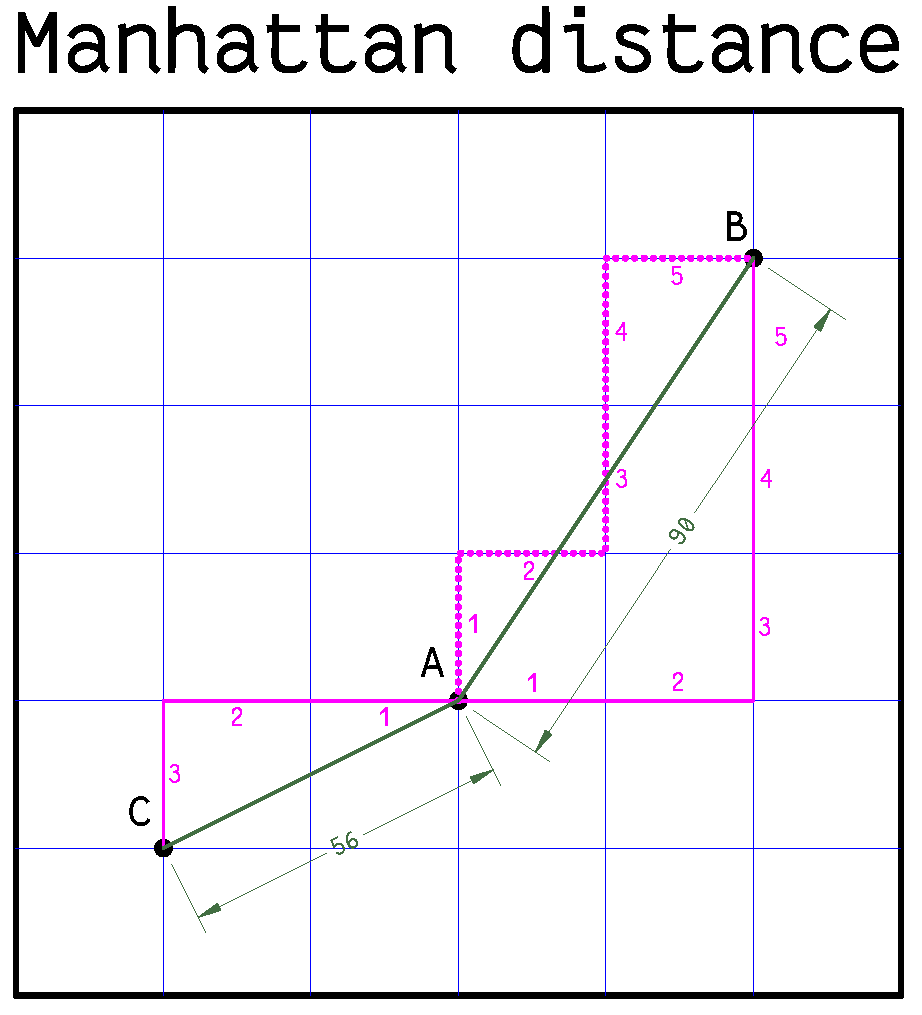
\includegraphics[width=0.75\textwidth]{Graphics/Manhattan}
\end{figure}

In the absolute sum (taxicab or Manhattan-) norm \(\ell_1 = ||\AbsVec{x}||_1 = \sum_{i=1}^n{|\AbsVec{x}_i|} \) the distance between two points is the sum of the absolute differences of their Cartesian coordinates. The name alludes to the grid layout of most streets on the island of Manhattan. A taxicab driving between two intersections drives the distance corresponding to the length of the \skalar{\ell_1}-norm (see fig. \ref{fig:Manh}).

\begin{lstlisting}[caption=Absolute sum norm]
  FUNCTION VectorAbsoluteSumNorm(CONST Vec: VectorTyp): float;

  VAR
    i: WORD;
    Sum: float;

  BEGIN
    IF (VectorLength(Vec) = 0)
      THEN
        BEGIN
          Result := 0;
          EXIT;
        END;
    Sum := 0;
    FOR i := 1 TO VectorLength(Vec) DO
      Sum := Sum + Abs(GetVectorElement(Vec, i));
    Result := Sum;
  END;
\end{lstlisting}

\subsubsection{Vector normalisation}

These are special cases of \skalar{p}-norms, \(||\AbsVec{x}||_p = \sqrt[p]{\sum_{i=1}^n{|\AbsVec{x}_i|^p}} \) for \(p = 1, 2, \infty \), respectively. Vectors can be normalised by dividing all elements by a norm:

\begin{lstlisting}[caption=Normalisation of vector]
  PROCEDURE NormaliseVector(VAR Vec: VectorTyp; Norm: float);

  BEGIN
    DivConstant(Vec, Norm);
  END;
\end{lstlisting}


\subsubsection{Inner (dot) product of a vector}\label{text:dotprod}

The inner product of two vectors \AbsVec{a,b} is a real number \(\AbsVec{a} \odot \AbsVec{b} = \sum_{i=1}^n{(\AbsVec{a}_i \AbsVec{b}_i)} \), the signed area of the parallelogram formed by the vectors. The sign depends on the angle between the vectors (clock- or counter-clockwise).  We use \Name{Neumaier}-addition to prevent the accumulation of error:

\begin{lstlisting}[caption=Inner product of vectors]
  FUNCTION VectorInnerProduct(CONST A, B: VectorTyp): float;

  VAR
    i, n1, n2: WORD;
    x: VectorTyp;

  BEGIN
    n1 := VectorLength(A);
    n2 := VectorLength(B);
    IF (n1 <> n2)
      THEN
        BEGIN
          CH := WriteErrorMessage('Vector error: Inner Product of vectors of unequal length');
          VectorError := true;
          EXIT;
        END;
    IF (n1 = 0)
      THEN
        BEGIN
          Result := 0;
          EXIT;
        END;
    CreateVector(x, n1, 0.0);
    FOR i := 1 TO n1 DO
      SetVectorElement(x, i, GetVectorElement(A, i) * GetVectorElement(B, i));
    Result := NeumaierSum(x);
    DestroyVector(x);
  END;
\end{lstlisting}

\subsubsection{Angle between two vectors}

The angle between two vectors is then calculated by \(\alpha = \frac{\AbsVec{ab}}{|\AbsVec{a}| |\AbsVec{b}|} \):

\begin{lstlisting}[caption=Angle between vectors]
  FUNCTION VectorAngle(CONST A, B: VectorTyp): float;

  VAR
    n1, n2: WORD;

  BEGIN
    n1 := VectorLength(A);
    n2 := VectorLength(B);
    IF (n1 <> n2)
      THEN
        BEGIN
          CH := WriteErrorMessage('Vector-Error: Angle between vectors of unequal dimension');
          VectorError := TRUE;
          EXIT;
        END;
    IF (n1 = 0)
      THEN Result := 0
      ELSE Result := ArcCos(VectorInnerProduct(A, B) /
        (VectorEuklidianNorm(A) * VectorEuklidianNorm(B)));
  END;
\end{lstlisting}

\texttt{TotalSum} and \texttt{TotalProduct} calculate the sum or product over all elements of the vector. Any \acs{NaN} is handled by ignoring that value. Therefore, to calculate the arithmetic or harmonic mean, one cannot simply use \texttt{VectorLength()} to determine the number of actual elements:

\begin{lstlisting}[caption=Number of non-NaN elements]
  FUNCTION ActualElements(CONST A: VectorTyp): WORD;

  VAR
    i, j: WORD;

  BEGIN
    j := 0;
    FOR i := 1 TO VectorLength(A) DO
      IF IsNaN(GetVectorElement(A, i))
        THEN
        ELSE INC(j);
    Result := j;
  END;
\end{lstlisting}


\subsection{Scaling, centering and normalisation of vectors}

To scale a vector to the range \([0\ldots 1] \) we can use
\begin{equation}
  \AbsVec{y} = \frac{\AbsVec{x} - \min{(\AbsVec{x})}}{\max{(\AbsVec{x})} - \min{(\AbsVec{x})}}
\end{equation}
If the data contain outliers, it can be useful to use, say, the 5th and 95th percentile instead of the minimum and maximum. For this reason, we give \texttt{min} and \texttt{max} as parameters of the function rather than determining it within:

\begin{lstlisting}[caption=Scaling a vector]
  PROCEDURE Scale(VAR Vec: VectorTyp; min, max: float);

  VAR
    i: WORD;
    Range: float;

  BEGIN
    Range := max - min;
    FOR i := 1 TO VectorLength(Vec) DO
      SetVectorElement(Vec, i, (GetVectorElement(Vec, i) - min) / Range);
  END;
\end{lstlisting}

A data vector is centered by subtracting the arithmetic mean, so that the new mean becomes zero:
\begin{equation}
  \AbsVec{y} = \AbsVec{x} - \bar{\AbsVec{x}}
\end{equation}


\begin{lstlisting}[caption=Centering a vector]
  PROCEDURE Centre(VAR Vec: VectorTyp);

  VAR
    Mean: float;
    i: WORD;

  BEGIN
    Mean := NeumaierSum(Vec) / ActualElements(Vec);
    FOR i := 1 TO VectorLength(Vec) DO
      SetVectorElement(Vec, i, GetVectorElement(Vec, i) - Mean);
  END;
\end{lstlisting}

\subsection{Vector distance}

The distance between two row vectors (observations) \Vector{a}, \Vector{b} is the sum of the squared differences \( \sum_{i=1}^n(\AbsVec{a}_i - \AbsVec{b}_i)^2 \):

\begin{lstlisting}[caption=]
  FUNCTION SquaredEuklidianDistance(CONST A, B: VectorTyp;
    IgnoreFirst: BOOLEAN): float;

  VAR
    p, i, start: WORD;
    c: CHAR;
    ai, bi, Sum: float;

  BEGIN
    p := VectorLength(A);
    IF VectorLength(B) <> p
      THEN
        BEGIN
          VectorError := TRUE;
          c := WriteErrorMessage('Euklidian distance of two vectors: vectors have unequal length');
          EXIT;
        END;
    Sum := 0;
    IF IgnoreFirst
      THEN Start := 2   // first column study number
      ELSE Start := 1;  // first column data
    FOR i := Start TO p DO
      BEGIN
        ai := GetVectorElement(A, i);
        bi := GetVectorElement(B, i);
        IF IsNaN(ai) OR IsNaN(Bi)
          THEN
            BEGIN
              VectorError := TRUE;
              c := WriteErrorMessage(
                'Euklidian distance of two vectors: vectors contain NaN');
              EXIT;
            END;
        Sum := Sum + Sqr(ai - bi);
      END;
    Result := Sum;
  END;
\end{lstlisting}



\section{Sorting a vector}\label{text:sort}

There are several different sorting algorithms, with different efficiencies with respect to memory requirement and computation speed. For medium numbers of elements (several hundred to a few thousand), the \Name{Shell} sort is often the best compromise, even if values are partially sorted already. This routine, modified from \parencite{Mor-13}, can handle \acs{NaN} elements and sorts them as highest values:
\begin{lstlisting}[caption=Shell sort]
  PROCEDURE ShellSort(VAR t: VectorTyp);

  LABEL
    10;

  VAR
    i, j, k, l, m, nn, NaNs, n, LdN: INTEGER;
    tmp, s: float;

  BEGIN
    NaNs := 0;
    s := -1e300;
    n := VectorLength(t);
    FOR i := 1 TO n DO
      BEGIN
        IF IsNaN(GetVectorElement(t, i))    // check FOR NaN data
          THEN INC(NaNs)
          ELSE IF (GetVectorElement(t, i)) > s
                 THEN s := GetVectorElement(t, i); // AND find largest element OF data vector
      END;
    s := 10 * s;
    IF (NaNs > 0)
      THEN
        FOR i := 1 TO n DO
          IF IsNaN(GetVectorElement(t, i))
            THEN SetVectorElement(t, i, s);
    // replace all NaN WITH very large number so they Move TO END OF vector
    LdN := Trunc(Ln(n) / Const_ln2);
    m := n;
    FOR nn := 1 TO LdN DO
      BEGIN
        m := m DIV 2;
        k := n - m;
        FOR j := 1 TO k DO
          BEGIN
            i := j;
  10:       l := i + m;
            IF (GetVectorElement(t, l) < GetVectorElement(t, i))
              THEN
                BEGIN
                  tmp := GetVectorElement(t, i);
                  SetVectorElement(t, i, GetVectorElement(t, l));
                  SetVectorElement(t, l, tmp);
                  i := i - m;
                  IF i >= 1 THEN GOTO 10;
                END;
          END;
      END;
    IF (NaNs > 0) THEN
      FOR i := Succ(n - NaNs) TO n DO  // change the top NaNs elements back TO NaN
        SetVectorElement(t, i, NaN);
  END;


  END.
\end{lstlisting}

\printbibliography[heading=subbibliography]
\end{refsection}

